%%
%% Skript Differentialgeometrie im Wintersemester 12/13
%% Zur Vorlesung von Dr. Grensing am KIT Karlsruhe
%%
%% Uebung 4
%%

\section{19. November 2012}
\setcounter{Aufg}{0} %Damit die Aufgaben jedes Mal bei Aufgabe 1 anfangen
\setcounter{Loes}{0}

\begin{Loes}
asdf
\end{Loes}

\begin{Loes}
Sei $\{U_\alpha | \alpha \in I\}$ eine offene "Uberdeckung vom $M$, $g_{\alpha\beta}: U_\alpha \cap U_\beta \to \GL(k,\R)$, $g_{\alpha\gamma}(p) = g_{\alpha\beta}(p) \cdot g_{\beta\gamma}(p)$ f"ur alle $ \in U_\alpha \cap U_\beta \cap U_\gamma$. Sei $E := \dot\bigcup_{\alpha \in I} (U_\alpha \X \R^k)_{/\sim}$, wobei f"ur $(p,v)_\alpha \in U_\alpha \X \R^k$, $(q,w)_\beta \in U_\beta \X \R^k$ gilt $(p,v)_\alpha \sim (q,w)_\beta \Leftrightarrow p=q$ und $v = g_{\alpha\beta}(p) \cdot w$.

\emph{Behauptung:} $\pi: E \to M$, $[p,v] \mapsto p$ ist ein Vektorb"undel.

\begin{description}[leftmargin=*]
\item[\quot{$\bm{\sim}$} ist "Aquivalenzrelation:]\begin{itemize}[leftmargin=*]
	\item
		$(p,v)_\alpha \sim (p,v)_\alpha$ gilt: $g_{\alpha\alpha}(p) = \Id v$ ($g_{\alpha\alpha}(p) = \underbrace{g_{\alpha\alpha}(p)}_{\mathclap{\in \GL(k,\R)}} \cdot g_{\alpha\alpha}(p)$)
	\item
		$(p,v)_\alpha \sim (q,w)_\beta \Rightarrow (q,w)_\beta \sim (p,v)_\alpha$ gilt: $p=q$, $v=g_{\alpha\beta}(p)w$ $\Rightarrow w = (g_{\alpha\beta}(p))^{-1} v = g_{\beta\alpha} v$ ($g_{\alpha\alpha}(p) = g_{\alpha\beta}(p) g_{\beta\alpha}(p)$)
	\item
		Transitivit"at folgt aus $g_{\alpha\gamma} = g_{\alpha\beta} g_{\beta\gamma}$
	\end{itemize}
\item[$\bm{E_p}$ ist $\bm{k}$-dimensionaler Vektorraum:]
	\[ [(p,v)_\alpha] + \lambda[(p,w)_\alpha] := [(p, v + \lambda w)_\alpha] \]
	\begin{description}[font=\normalfont\itshape,leftmargin=*]
	\item[unabh"angig von $\alpha$:]
		\begin{align*}
			[(p,v)_\beta] + \lambda[(p,w)_\beta] &= [(p,g_{\alpha\beta}(p)v)_\alpha] + \lambda[(p,g_{\alpha\beta}(p)w)_\alpha] \\
				&= [(p,g_{\alpha\beta}(p)v + \lambda g_{\alpha\beta}(p)w)_\alpha] \\
				&= [(p,g_{\alpha\beta}(p) \cdot(v + \lambda w))_\alpha] = [(p,v + \lambda w)_\beta]
		\end{align*}
	\item[$k$-dimensional:]
		$q|_{\{p\} \X \R^k} : \{p\} \X \R^k \to E_p$ ist Vektorraum-Isomorphismus (wobei $q: \dot \bigcup_{\alpha \in I} (U_\alpha \X \R^k) \to E$)
	\end{description}
\item[B"undelkarten (glatt):]
	$\Phi_\alpha: U_\alpha \X \R^k \to E|_{U_\alpha}$, $(p,v) \mapsto [(p,v)_\alpha]$ ist Hom"oomorphismus, da $\sim|_{(U_\alpha \X \R^k) \X (U_\alpha \X \R^k)}$ die triviale "Aquivalenzrelation ist.
	\begin{align*}
		\Phi_\alpha \circ \Phi_\beta^{-1}(p,v) &= \Phi_\alpha([(p,v)_\beta])\\
		&= \Phi_\alpha([(p,g_{\alpha\beta}(p)v)_\alpha])\\
		&= (p, g_{\alpha\beta}(p)v)
	\end{align*}
	$\Rightarrow \Phi_\alpha \circ \Phi_\beta^{-1}$ ist glatt. $\Phi_\alpha|_{E_p}$ ist Vektorraum-Isomorphismus.
\item[\quot{normale} Karten:]
	Sei $\phi$ Karte von $M$ mit Kartengebiet $U \subset U_\alpha$ $\leadsto$ $\overline\phi_\alpha: E|_U \to \phi(U) \X \R^k$, $e \mapsto (\phi(\pi(e)), (\Phi_\alpha)^2(e))$.
	
	Glatte Kartenwechsel $\checkmark$
\item[$\bm{E}$ Hausdorffsch:]
	$[(p,v)_\alpha] \ne [(q,w)_\beta] \in E$
	\begin{description}[font=\normalfont,leftmargin=*]
	\item[$p\ne q$:]
		Die Urbilder in $M$ trennender Umgebungen von $p$ und $q$ unter $\pi$ trennen die Punkte in $E$.
	\item[$p=q$:]
		$v \ne g_{\alpha\beta}(p) w$ $\leadsto$ trennen im $\R^k$ und "uber $\Phi_\alpha$ zur"uckziehen.
	\end{description}
\item[abz"ahlbare basis der Topologie (f"ur $\bm{U_{\alpha}} \bm{\X} \R^{\bm{k}} \bm{\checkmark}$):]
	Es gibt ein $I ' \subseteq I$ mit $I$ abz"ahlbar und $M = \bigcup_{\alpha \in I'} U_\alpha$. Sei $\{V_j | j \in J'\}$ abz"ahlbare Basis der Topologie von $M$. Dann ist mit $J = \{j \in J' | V_j \subset U_\alpha \text{ f"ur ein } \alpha \in I\}$, $\{V_j | j \in J\}$ auch abz"ahlbare Basis der Topologie von $M$, denn $U \underset{\mathclap{\text{offen}}}{\subset} M$ $\Rightarrow$
	\begin{align*}
		U &= \bigcup\limits_{\alpha \in I} (U_\alpha \cap U) \\
		&= \bigcup\limits_{\alpha \in I} \bigcup\limits_{\substack{j \in J' \\ U_j \subset U_\alpha \cap U}} V_j \tag{$U_j \subset U_\alpha \cap U \Rightarrow j \in J$} \\
		&= \bigcup\limits_{\alpha \in I} \bigcup\limits_{\substack{j \in J \\ V_j \subset U_\alpha \cap M}} V_j
	\end{align*}
	F"ur $j \in J$ sei $\alpha(j) \in I$, sodass $V_j \subset U_{\alpha(j)}$. Setze $I' := \{ \alpha(j) | j \in J\}$.
		\[ \bigcup_{\alpha \in I'} U_\alpha = \bigcup_{j \in J} U_{\alpha(j)} \supseteq \bigcup_{j \in J} V_j = M \]
\end{description}\end{Loes}

\begin{Loes}
Es seien $E, E'$ Vektorb"undel "uber $M$ und $F: E \to E'$ sei ein B"undelmorphismus mit dem Isomorphismus $F_p: E_p \to E_p'$ f"ur alle $p \in M$.

\emph{Behauptung:} $F$ ist ein B"undelisomorphismus

$F$ ist surjektiv, denn f"ur $e \in E'$ ist $F_{\pi'(e)}: E_{\pi'(e)} \to E'_{\pi'(e)}$ bereits ein Isomorphismus, also existiert ein Urbild $\tilde e \in E_{\pi'(e)} \subset E$ mit $F(\tilde e) = F_{\pi'(e)}(\tilde e) = e$. Dass $F$ injektiv ist folgt analog, da $\pi' \circ F = \pi$.

Damit existiert ein $G: E' \to E$ mit $G \circ F = \Id$, $F \circ G = \Id$ und $\pi \circ G = \pi'$. Damit gilt auch
	\[ G(e') = (F_{\pi'(e)})^{-1}(e') \]
Es sei nun ein offenes $U  \subseteq M$ mit den Trivialisierungen $E|_U$ und $E'|_U$ gegeben.
\begin{center}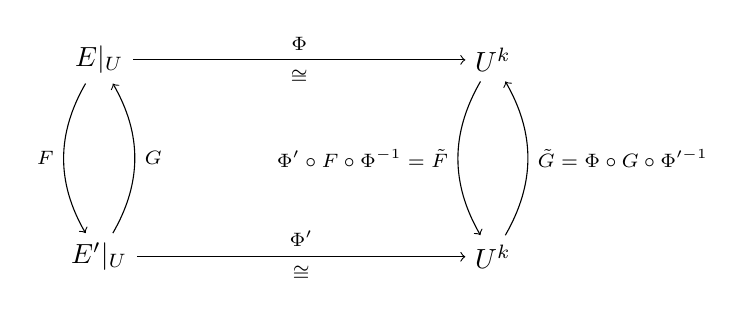
\begin{tikzpicture}
	%\draw[step=0.25,gray!15] (-4,-4) grid (4,4); \draw[step=0.5,gray!30] (-4,-4) grid (4,4); \fill (0,0) circle(0.1); %Hilfsgitter
	
	\def\hor{2.5}
	\def\vert{1.25}
	\def\angle{30}
	\node (1) at (-\hor,\vert) {$E|_U$}; \node (2) at (\hor,\vert) {$U \X \R^k$}; \node (3) at (-\hor,-\vert) {$E'|_U$}; \node (4) at (\hor,-\vert) {$U \X \R^k$};
	
	\draw[->] (1) --node[font=\scriptsize,above]{$\Phi$}node[font=\scriptsize,below]{$\cong$} (2);
	\draw[->] (3) --node[font=\scriptsize,above]{$\Phi'$}node[font=\scriptsize,below]{$\cong$} (4);
	
	\draw[->] (1) to[out=270-\angle,in=90+\angle]node[left,font=\scriptsize]{$F$} (3);
	\draw[->] (3) to[out=90-\angle,in=270+\angle]node[right,font=\scriptsize]{$G$} (1);
	
	\draw[->] (2) to[out=270-\angle,in=90+\angle]node[left,font=\scriptsize]{$\Phi' \circ F \circ \Phi^{-1} = \tilde F$} (4);
	\draw[->] (4) to[out=90-\angle,in=270+\angle]node[right,font=\scriptsize]{$\tilde G = \Phi \circ G \circ \Phi'^{-1}$} (2);
\end{tikzpicture}\end{center}
Da $\pi' \circ F = F$ ist, existiert eine Abbildung $f: U \to \GL(k, \R)$ sodass $\tilde F(p,v) = (p, f(p) \cdot v)$ ist. Daraus folgt dass $\tilde G(p,w) = (p, (f(p))^{-1}w)$ glatt ist, da $\cdot^{-1}: \GL(k,\R) \to \GL(k, \R)$ glatt ist (denn $A^{-1} = \frac{1}{\det A}((-1)^{i+j} \det A[i,j])_{i,j}^T$). Damit ist $G$ glatt und somit auch ein B"undelmorphismus.
\end{Loes}

\begin{Loes}\begin{enumerate}[label=(\alph*),leftmargin=*,widest=a]
\item
	\emph{Behauptung:} Es sei $E$ ein Vektorb"undel vom Rang $k$ "uber $M$ auf dem $k$ punktweise linear unabh"angige Schnitte existieren. Dann ist $E$ trivial.
	
	Es seien $\sigma_1, \ldots, \sigma_k: M \to E$ Schnitte, die punktweise linear unabh"angig sind. Dann hat $E_p$ als Basis $\sigma_1(p),\ldots ,\sigma_k(p)$. Definiere nun $F: E \to M \X \R^k$, $\sum_{i=k}^k a_i \sigma_i(p) \mapsto (p, a_1,\ldots ,a_k)$. Es gilt $\pi_1 \circ F = \pi$ und $F_p$ ist ein Isomorphismus. $F$ ist glatt, denn f"ur eine B"undelkarte $\Phi$ ist $\tilde \sigma_i = \Phi^2 \circ \sigma_i$\marginnote{\scriptsize{$\Phi^2$ ist die zweite Komponente}}, das hei"st $\Phi(\sigma(p)) = (p, \tilde\sigma(p))$. Mit $A(p) = (\tilde\sigma_1(p),\ldots ,\tilde\sigma_k(p))^{-1}$ gilt:
	\[ F \circ \Phi^{-1}(p,v) = (p, A(p) \cdot V) \]
Daher ist $F$ glatt und mit Aufgabe 3 folgt, dass $F$ ein B"undelmorphismus ist.
\item
	\emph{Zu zeigen:} $\T S^3 \cong S^3 \X \R^3$
	
	Es gilt:
		\[ \T_pS^3 \cong p^\perp \ni \underbrace{\begin{pmatrix} -p_2 \\ p_1 \\ -p_4 \\ p_3 \end{pmatrix}}_{=:\sigma_1(p)} \cdot \underbrace{\begin{pmatrix} p_3 \\ -p_4 \\ -p_1 \\ p_2 \end{pmatrix}}_{\sigma_2(p)} \cdot \underbrace{\begin{pmatrix} -p_4 \\ -p_3 \\ p_2 \\ p_1 \end{pmatrix}}_{\sigma_3(p)} \]
	Dadurch sehen wir dass $\sigma_i(p) \perp \sigma_j(p)$ f"ur $ i \ne j$, woraus folgt dass $\sigma_1, \ldots ,\sigma_3$ punktweise linear unabh"agige Schnitte sind. Mit (a) folgt dann die Behauptung.
\end{enumerate}\end{Loes}

\begin{emptythm}[Anmerkung]
Der Raum der Schnitte $\Gamma(M,E)$ ist ein $\R$-Vektorraum, also ist lineare Unabh"angigkeit f"ur Schnitte definiert. Linear unabh"angige Schnitte sind im Allgemeinen \emph{nicht} punktweise linear unabh"angig. Betrachte beispielsweise
	\[ \pi_1: \underset{\mathclap{\text{\textcolor{gray}{Mf.}}}}{\R} \X \underset{\mathclap{\text{\textcolor{gray}{VR}}}}{\R} \to \R \]
Dann sind $\sigma_1(t) = (t,1)$ und $\sigma_2(t) = (t,t)$ lineare unabh"angig, aber in jedem Punkt linear abh"angig.
\end{emptythm}